%% Exemple de source LaTeX pour un article soumis à TALN
\documentclass[10pt,a4paper,twoside]{article}

\usepackage[utf8]{inputenc}
\usepackage[T1]{fontenc}
\usepackage{graphicx}

% Package utilisé uniquement pour l'exemple.
\usepackage{lipsum}
\usepackage{hyperref}

% faire les \usepackage dont vous avez besoin AVANT le \usepackage{jeptaln2012} 
% add the \usepackage for you packages BEFORE the \usepackage{jeptaln2012}

\usepackage{talnrecital2013}
% Insérer les définitions de biblio en français (cf apalike-fr.bst)
\usepackage[frenchb]{babel}

\title{Bases lexicales multilingues : traitement des acronymes}

\author{Ying Zhang\up{1}\quad Mathieu Mangeot\up{1}\\
{\small  (1) GETALP-LIG, 41 rue des mathématiques  BP 53 38041 Grenoble Cedex 9\\ 
  \texttt{ying.zhang@imag.fr, mathieu.mangeot@imag.fr} \\ 
}}

\begin{document}

\maketitle

%% In an English article, use \resumeEn with 2 arguments (french title and french summary)
\resume{
La gestion des terminologies est un domaine de recherche à long terme. En particulier pour les situations compliquées comme les acronymes, la recherche n’est jamais interrompue. Dans cet article, nous parlerons de lier plusieurs termes différents à un seul référent via les notions de pivot et de prolexème. Ces notions permettent par exemple de faire le lien entre plusieurs termes qui désignent un même et unique référent : nations unies, ONU, organisation des nations unies et onusien. Il existe Jibiki, une plate-forme générique de gestion de bases lexicales permettant de gérer n’importe quel type de structure (macro et microstructure). Nous avons implémenté la notion de prolexème[…] dans la plate-forme Jibiki pour réaliser les gestions des terminologies riches comme les acronymes.
}

%% In an English article, use \abstractEn with 1 arguments (english summary)
\abstract{TALN-RECITAL2013 template (English translation of the article title)}{
The translation of the title in English is mandatory to enhance visibility of the online version of the papers in international scientific article databases (DBLP, citeseer, etc.). Here an abstract in English (max. 150 words).\\
}

\motsClefs{base lexicale multilingue, macrostructure, Jibiki, Pivax, Common Dictionary Markup, iPoLex, entrepôt de données linguistiques}
{multilingual lexical database, macrostructure, Jibiki, Pivax, Common Dictionary Markup, iPoLex, linguistic data warehouse}

%\motsClefs{Ici une liste de mots-clés en français}
%{Here a list of keywords in English}

%% Aller à la page suivante si nécessaire
%\newpage
%%================================================================
\section{Introduction}

\subsection{Situation}
L

\subsection{Intérêt}

L

\subsection{Présentation}

L

\section{Problématique}

% reprendre l'explication du cahier des charges des acronymes
Les liens entre les termes sont compliqués. Il existe la possibilité de lier plusieurs termes différents à un seul référent : Jean‐Paul II et Karol Jozef Wojtyla en français, ou en anglais John Paul II et Karol Jozef Wojtyla. De même, certains liens évoluent avec le temps : le pape désignait Jean­‐Paul II en 2004 et Benoît XVI en 2012. Des pays parlant la même langue (ex : France et Suisse romande) peuvent également utiliser des mots différents pour le même concept. Ex : "chien renifleur" et "chien drogue". Inversement, le même terme peut désigner des concepts différents : Dans la province de langue allemande de Bolzano en Italie, le Landeshauptmann est le président du conseil provincial, avec des compétences beaucoup plus limitées que le Landeshauptmann autrichien, qui est à la tête de l'un des Etats (Land) de la fédération autrichienne.\\
Pour les gestions des acronymes, les liens riches sont plus répandu et plus complexe. Dans l'article introduisant la notion de Prolexème, il a été discuté qu’il y a des lexies ayant des acronymes dans certaines langues, mais pas dans d'autres. Par exemple, en français, il y a « organisation des nations unies », on peut aussi dire « Nations unies », « ONU », « onusien ». En anglais, on a « United Nations » et son acronyme « UNO ». En chinois, on a 联合国 qui est la seule lexie pour cette signification, et il n’y a pas d’acronyme. Quand on construit des ressources lexicales, comment créer les liens entre les acronymes et les mots standard ?\\
Dans les chapitres suivants, nous parlerons des idées pour résoudre les problèmes décrits ci-dessus. 

\section{Données : choix de la macrostructure}

% dans cet article, on ne détaille pas la microstructure. On l'évoquera seulement
La macrostructure est la structure de dictionnaire, il est l’organisation des volumes. Les volumes sont les ressources lexicales, un dictionnaire comprend un ou plusieurs volumes.\\
Nous avons plusieurs types de macrostructure qui correspond aux les types différents de dictionnaire.  Ici, nous présenterons trois macrostructures principales.\\

\subsection{Macrostructure Papillon}

% utilise le concept de lexies (TST, Mel'cuk)
% présente le concept de structure pivot et d'axie
L \cite{GSMM01a}

\subsection{Macrostructure Pivax}

% présente le concept d'axème, de multiples volumes dans la même langue et de structure pivot à étages
L \cite{MMHTN09}

\subsection{Macrostructure ProAxies}

% utilise les concepts présentés précédemment (structure pivot à étages, multiples volumes dans la même langue, lexies, axies, axemes)
% utilise le concept de prolexème (au même niveau que les axèmes)
% présente le concept de proaxie
\begin{figure}[htbp] 
\begin{center} 
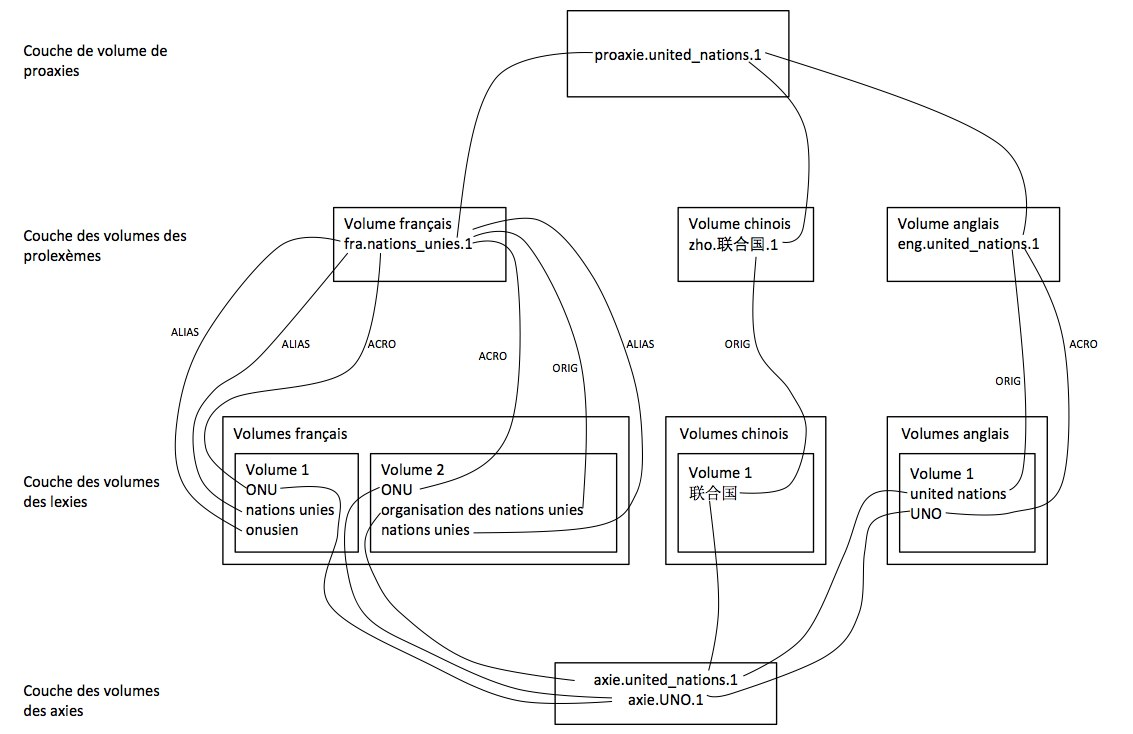
\includegraphics[width=14cm]{images/proaxie.jpg}
\end{center} 
\caption{Macrostructure de ProAxie} \label{image} \
\end{figure}


\section{Outils nécessaires : plateformes de manipulation}

\subsection{Plateforme Jibiki v1}

% parle des différents outils existants : tswanelex, DPC, voir
\cite{MMCE11}
% présente la plateforme : CDM et table d'index, édition générique, opensource, licence GPLv3, dispo publiquement et gratuitement sur ligforge en SVN, sert pour de multiples projets
% explique les limitations : pas de liens entre plusieurs volumes différents, macrostructures complexes (pivot, pivax, etc.) codées en dur, difficultés de création de méta-données

\cite{MMAC06}

\subsection{Gestion des données et méta-données : iPoLex}

% explique le concept d'entrepôt de données
% génération assistée des méta-données

\subsection{Gestion des liens riches : extension Jibiki-Pivax}

% explique la nouvelle gestion des liens riches : 
% liens : volume de destination, poids, type (axi, final), langue, étiquette libre, etc. 
% table de liens séparée
% algorithme de collecte des liens dans DictionariesFactory.java (expandResults)
% algorithme de construction du résultat : parcours montant vers les axies puis descendant vers les lexies cibles

\section{Résultats préliminaires}

% montre les résultats de recherche pour différents scénarios

% scénario 1 : montre si une axie est dispo ONU => ONU en chinois 
% scénario 2 : montre s'il n'y a pas d'axie de dispo, on passe par la proaxie et on utilise l'étiquette (label) Organisation des Nations Unies => United Nations
% scénario 3 : montre s'il n'y a pas d'axie de dispo et pas d'étiquette correspondante. On utilise seulement la proaxie : Trouver un exemple avec un acronyme dans une langue et pas dans une autre (onusien vers chinois et vers anglais )

\section{Conclusion}

L

% à effacer à la fin
\section{Exemples à effacer à la fin}

\begin{itemize}
\item Une liste à puce
\item avec plusieurs lignes
\item pas trop espacées... 
\end{itemize}

\begin{enumerate}
\item Une liste numérotée
\item où le 2. succède, étrangement, au 1.
\item et le trois, au deux... (ce serait pas ambigu cela ?)
\end{enumerate}

\subsubsection{Figures et tables}

Les figures et les tables seront centrées sur la page avec une légende située en dessous. La légende contiendra le mot clé figure (ou table) en petite capitale, suivi du numéro de la figure ou de la table (numéros indépendants). La figure \ref{image} et la table \ref{table} en sont un exemple. Les équations peuvent figurer "en ligne" ou centrées sur la page, sans légende. Un numéro de renvoie peut figurer à droite de l'équation pour permettre les références dans le texte.

\begin{table}[!h]
\centering
	\begin{tabular}{|c|p{4cm}|}
	\hline
	Un tableau&\\
	\hline
	&Les cellules ainsi que le tableau sont centrés\\
	\hline
	\end{tabular}
\caption{Un tableau}\label{table}
\end{table}

\begin{figure}[htbp] 
\begin{center} 

\includegraphics{images/atala.png}
\end{center} 
\caption{Une image comme figure} \label{image} \
\end{figure}
Paragraphe facultatif

%%================================================================
%% Note : si l'on préfère éviter de factoriser les crossrefs :
%% bibtex -min-crossrefs 99 taln-exemple
%%================================================================

\bibliographystyle{apalike-fr}
\bibliography{biblio-mangeot}

%%================================================================
\end{document}
